% !TEX encoding = Mac Central European Roman
\documentclass[a4paper,12pt]{article}

\usepackage{amsmath, amssymb, mathtools, verbatim, bm, xcolor, hyperref}
%\usepackage[polish]{babel}
%\usepackage{polski}
\usepackage[T1]{fontenc}
\usepackage[utf8]{inputenc}
\usepackage{textcomp}
%\usepackage[macce]{inputenc}
%\usepackage[latin2]{inputenc}
\usepackage{epigraph}
\usepackage{physics}
\usepackage[textsize=tiny]{todonotes}
\definecolor{lightgray}{gray}{0.90}
\newtheorem{theorem}{Theorem}
\usepackage{framed}
\renewenvironment{leftbar}[1][\hsize]
{% 
\def\FrameCommand 
{%

    {\hspace{-3pt}\color{black}\vrule width 3pt}%
    \hspace{0pt}%must no space.
    \fboxsep=\FrameSep\colorbox{lightgray}%
}%
\MakeFramed{\hsize#1\advance\hsize-\width\FrameRestore}%
}
{\endMakeFramed}
\setlength{\FrameSep}{0pt}

%\usepackage{showframe}
\usepackage[left=70pt,
			right=70pt,
            top=50pt,
%            textwidth=345pt,
            marginparsep=0pt,
            marginparwidth=70pt,
%            textheight=692pt,
%            footskip=50pt
            ]
           {geometry}
%\textwidth=16.5 truecm
%\textheight=25 truecm
%\hoffset=-2.5 truecm
%\voffset=-2 truecm

\def\baselinestretch{1.2}

%\pagestyle{empty}

\begin{document}

\title{Non-equilibrium systems and growth of complexity}

\author{Michał Mandrysz \\
Instytut Fizyki, Uniwersytet Jagielloński, \\ul. Łojasiewicza
11, 30-348 Kraków, Polska }



\maketitle

\tableofcontents

\newpage
\epigraph{True logic of this world lies in the calculus of probabilities}{\textit{James Clerk Maxwell}}

\section{Historical introduction}
\subsection{The founding fathers of thermodynamics}
The history of thermodynamics reaches back to the 1600s when first rudimentary thermoscopes (the ancestor of the thermometer) started to be constructed and a scientists, like Francis Bacon began to formulate the right ideas about the nature of heat. 

It took however until 1850s, after the experiments of James Joule, for the wide scientific community to finally accept heat as a form of energy. The relation between heat and energy was important for the development of steam engines and led to the description of idealized heat engines and their theoretical efficiency in 1824 by Sadi Carnot. 

After that, around 1850 Rudolf Clausius and William Thomson (Lord Kelvin) stated both the First Law (the conservation of total energy) as well as the Second Law (heat does not spontaneously flow from colder to hotter objects). Other formulations followed quickly and the general implications of the laws were understood. 

More important developments came after the recognition by Rudolf Clausius and James Clerk Maxwell in 1850s (first noticed by Daniel Bernoulli in 1738) that gases consist of molecules at motion. This simple idea allowed Maxwell to derive and calculate many macroscopic properties of gases at equilibrium. 

Shortly after that, Rudolf Clausius introduced the notion of entropy, defined as the ratio of heat and temperature and redefined the Second Law stating that for isolated systems this quantity can only increase in time.
%TODO: Describe the problem with defining the temperature

In 1872 Ludwig Boltzmann constructed an equation that he thought could describe the detailed time development of any gas and used it to derive the so-called H-theorem. The theorem stated that a quantity equal to entropy must always increase in time. Therefore it seemed that Boltzmann had successfully proved the Second Law. During his times however, a famous objection was poised known as the Loschmidt paradox which stated basically, that due to time-reversal property of Newton laws the evolution could be run in reverse leading to decrease in entropy. 

The resolution of this paradox was noted much later and should probably classified as hard to grasp or at least hard to get accustomed to because even today one can find discussions and erroneous statements about the "arrow of time" in the literature. Indeed, those difficulties were noted by Gibbs as well\cite{Gibbs:1928tw}:
“Any method involving the notion of entropy, the very existence of which depends on the second law of thermodynamics, will doubtless seem to many far-fetched, and may repel beginners as obscure and difficult of comprehension.” 
We will intentionally postpone the discussion to the later part of this paragraph in order to go through it thoroughly and to highlight the more recent paths of developments in non-equilibrium thermodynamics and statistical physics.

In responding to some of the other objections Boltzmann realized around 1876 that in a gas there are many more states that seem chaotic and random than seem orderly. This realization led him to argue that entropy must be proportional to the logarithm of the number of possible states of a system and the nature of the Second Law - probabilistic.

Around 1900, Williard Gibbs formulated statistical mechanics in more general context and introduced the notion of ensemble - a collection a collection of many macroscopically similar copies of the system upon which the notion of ergodicity was built. 
It was argued that if a single particle visits every possible piece of the phase space, then when averaged over a sufficiently long time then a property in question would have the same value if one would instead think of ensembles. 

Gibbs also introduced another definition of entropy, which, as noted by him \cite{Gibbs:1962bk} would only increase in a closed system if it were measured in a "coarse-grained" way in which nearby states were not distinguished. In literature one can sometimes find statements \cite{Evans:2016tq} that this property of Gibbs entropy is problematic, but in fact the resolution of this paradox in very similar to the resolution of the Loschmidt paradox.

During the beginning of the XX century, the development of thermodynamics was largely overshadowed by quantum theory and little fundamental work was done on it. 
Nevertheless, the Second Law had become to be regarded as a fundamental principal, whose foundations should be questioned only as a curiosity. Ergodic theory on the other hand has became an active area of pure mathematics, and between 1920-1960 many properties of simple systems related to ergodicity were established \cite{Wolfram:552851}.

\subsection{The information era and Schrödingers influence on physics}

In the 1940s Claude Shannon introduced the notion of information quantity and during the 1950s, it was recognized that entropy is simply the negative of Shannon's quantity. This way a fundamental link between information theory and thermodynamics was established. This coincided with the discovery of the structure of DNA by James Watson and Francis Crick and together with written a little earlier, influential book titled "What is life?" by  Erwin Schrödinger sparked enthusiasm and inspired generations of physicists to answer the alluring (though not easy) question of the role of physics in biological processes. 

In any event it probably wouldn't be an exaggeration to say that Schrödinger himself (as he admits), was inspired by the work of German-American physicists Max Delbrück; who helped launch the molecular biology research program in the late 1930s and explained (in main part) the mechanism of heredity and mutation.
Regardless, Schrödinger makes some very essential observations on the nature of living organisms.

First, their operation (living organisms) as a macroscopic system resembles approximately, a purely mechanical system rather than a thermodynamical system. 
Even though their size is far from what is considered a thermodynamic limit, they tend stay unaffected (in special environments) by random molecular motion known as heat and; at the same time, evade the decay towards equilibrium for an unusually long time. This is essentially the definition of a living system.

Secondly, he notices that the way an organism accomplishes the above is through the exchange of energy and matter with it's environment, that leaves it's own internal state in low entropy. He withdraws from considerations of free energy, although he acknowledges that the exact physical understanding should be accomplished through it rather than through entropy. Worth mentioning is his hypothesis of "life intensity" the term which ought to parallel with the rate at which the system produces entropy or dissipates heat.

Thirdly, each cell depends on very small group of atoms, the genetic code, which determine it's evolution, something unprecedented, beyond the description of ordinary statistical physics. He proposes, that perhaps, a partial explanation for this dynamical behaviour (rather than statistical) can be traced to rigidity and tightness of chemical bonds. However the very vital point Schrödinger tries to make is the hypothesis, that there must exist a yet unknown, new law of physics that would explain fully how order can be produced out of order. 

Lastly, even though Schrödinger introduces some quantum mechanics principles, like the uniqueness of Heitler-London bond in order to defend the theory laid down by Delbrück, he assures that quantum indeterminacy should play only marginal role in the future laws of dynamics of living systems. The possibility that remains is that the origins of life, not their evolution could be quantum mechanical.

As mentioned earlier, Schrödinger influence driven many researchers to focus on the topic of non-equilibrium phenomena, however their individual approaches diverged widely, due to, as we will see the resolution of the Loschmidt paradox.

\subsection{The resolution of the Loschmidt paradox }

The Loschmidt paradox confronts the fact that the fundamental equations of motion are time-reversible. How therefore the irreversibility enters the picture?

The answer lies in the time-asymmetric probabilistic way in which we make predictions about the world. 
Besides the pure probabilistic description we need the common sense, axiom of causality in order to obtain the time-asymmetric description.
We use it so frequently implicitly, that we often forget about it \cite{Evans:2016tq}. 

Indeed, Boltzmann himself didn't noticed that the way in which he derived the H-Theorem from his equation, implicitly assumed that the particles are uncorrelated before the collisions, but become correlated after the collision\cite{Dorfman:ozm67-zD}\cite{Wolfram:552851}, thus causing the time-reversal asymmetry.

One can also see this most clearly in a generic example, reviewing the procedure in which we compute some future macroscopic state from an initial state macrostate. The final state is obtained by taking the \textit{sum} of the probabilities over the indistinguishable microstates, however the initial state is obtained by taking the \textit{avarage} over the initial microstates.

\subsection{Different approaches towards irreversibility and non-equilibrium}

As one might tell from the large amount of literature on the subject \cite{Doyle:wf} \cite{Layzer:1970dx} \cite{Wolfram:552851} \cite{Rovelli:2015tv} \cite{Courbage:1983eo} %TODO: Add more citations
 that this explanation of irreversibility noticed long time ago by Boltzmann, Kelvin, Maxwell \cite{Wolfram:552851} and also Einstein (in the polemic with Ritz over time-reversal symmetry of Maxwell equations) still leaves dissatisfaction in many.

Different alternatives for explanations of irreversible processes have been proposed over the years, including fluctuations, randomness of the radiative process, quantum mechanics, CP violation, cellular automata and even gravity. We now will shortly discuss each of those approaches, starting our discussion from the most direct one, given Ilya Prigogine.

The motivation for such development was clearly articulated by Prigogine:
"I have always found it difficult to accept this conclusion [macroscopic irreversibility emerging from initial conditions] {...} especially because of the constructive role of irreversible processes. Can dissipative structures be the result of mistakes?" \cite{Prigogine:1978kz}.

His personal dissatisfaction with lack of irreversibility and unitary evolution at the microscopic level led him to postulate the existence of microscopic representation of entropy in the equations of motion. 
In essence, the idea was to change the fundamental laws of physics as to make them irreversible at the microscopic level. The details of this approach, known in literature as Misra-Prigogine-Courbage theory\cite{Courbage:1983eo}, will not be presented here, as in so far no evidence for its validity has been found\cite{Bricmont:7zJsfTpK}.

Some authors \cite{Doyle:wf}, stated that irreversibility enters

Classical statistical physics (with its Maxwell-Boltzmann distribution and other insights) was replaced by quantum statistical physics (with its Bose-Einstein and Fermi-Dirac distributions and similar wisdom). But both of these disciplines imply pretty much the same large N limit called thermodynamics. In the quantum case, the large N limit also includes the classical limit. The qualitative relation between thermodynamics on one side and statistical physics on the other side is pretty much identical in the classical and quantum world.

Another simple way to debunk the myth is to notice that the strength of all quantum phenomena is controlled by Planck's constant which is very tiny in "everyday units" while the manifestations of the arrow of time - such as friction - are clearly macroscopically large. So they can't be proportional to Planck's constant: their essence can't depend on quantum mechanics.

Other approaches to irreversible process mentioned earlier, most likely also fail.

including fluctuations, randomness of the radiative process, quantum mechanics, CP violation, cellular automata and even gravity

To summarise ...

\subsection{Physics of computation}

Following statements by John von Neumann, it was thought that any computational process must necessarily increase entropy,  but by the early 1970s, notably with work by Charles Bennett, it became accepted that this is not so (see page 1023), laying some early groundwork for relating computational and thermodynamic ideas. 

\subsection{Jaynes formulation of statistical mechanics}

The essence of MaxEnt method can be summarized in the formula for maximization of relative entropy (negative Kullback-Leibler divergence)

\begin{displaymath}
  H(p\lor q) = -\sum_i \ln p_i \frac{p_i}{q_i}
\end{displaymath}
with respect to $p_i$ (new aposteriori distribution). $H(p||q)$ can be interpreted as the information gained by using $p_i$ instead of $q_i$.


\section{Treatment of entropy in standard contexts}

\subsection{Gibbs entropy}

In comparison to Boltzmann entropy, Gibbs entropy is well defined also for a system of interacting particles \cite{Jaynes:1965gg}.

%TODO: Add Jaynes - Gibbs vs Boltzmann Entropies

In Hamiltonian systems Gibbs entropy stays constant.
The constancy of entropy in Hamiltonian systems was first discovered by Gibbs in 1903 and was commented on extensively but inconclusively by Ehrenfest review of the foundations of statistical mechanics.

That however doesn't mean that the concept of Gibbs entropy 
is useless.

%TODO: Proof from page 43

\subsubsection{Simple model}
Let's consider a model consisting of three elements: the cooler $C$, the heater $H$ and the system under consideration $S$, staying out of equilibrium.
We assume, that the temperatures of the cooler and the heater stay constant, and that heat $Q_H$ flows into the system $S$ and heat $Q_C$ flows out. The situation is illustrated by the picture \ref{Fig2}.
\begin{figure}[ht!]
\centering 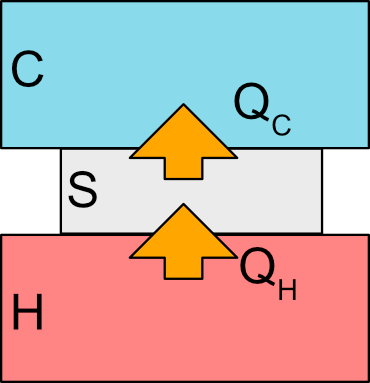
\includegraphics[width=6cm]{system} \caption{System (S) model}
\label{Fig2} 
\end{figure}

Treating the heater and the cooler as the environment, we can think of our system $S$ as an open system.
Further on we'll analyze the system $S$ from the perspective of internal $(i)$ entropy production
and external $(e)$ entropy flux, flowing \emph{to} the system $S$. 
Of course the change in entropy will be the sum of those two contributions:
\begin{equation}
dS_S=dS_i+dS_e.
\label{entrosum}
\end{equation}

In the current analysis let's consider a situation in which the same amount of heat flows in as flows out, that is $dQ_C=-dQ_H$. Using this relation we get the following term for the change of entropy:
\begin{equation}
dS_e=\frac{dQ_H}{T_H}+\frac{dQ_C}{T_C}=dQ_H\left(\frac{1}{T_H}-\frac{1}{T_C}\right)
=dQ_H\left(\frac{T_C-T_H}{T_HT_C}\right)<0.
\label{dSe1}
\end{equation}
From which it follows, that the heat flow takes the entropy out of our system.
For the purpose of further discussion we introduce the concept of rate of entropy change connected with the heat flow:
\begin{equation}
j_e \equiv  \frac{dS_e}{dt}. 
\end{equation}
In the considered scenerio, the $j_e$ is held constant (steady-state) and we suspect a continuous fall in system's entropy

Yet, moving away from the equilibrium state we suspect, that the a major role will be played by $dS_i$ moving the system back to equilibrium state. Similarly, as before we define the rate of internal entropy production:

\begin{equation}
j_i \equiv \frac{dS_i}{dt}.   
\end{equation} 

When $T_H=T_C$, i.e. the system is in equilibrium with constant entropy $S_{EQ}$ then it follows that $j_i=0$.
Therefore the rate of internal entropy production $j_i$ should be a function  of system's entropy $S_S$, i.e. $j_i = j_i(S_S)$ with the boundary condition $j_i(S_S=S_{EQ})=0$. 

Near the equilibrium state $S_S=S_{EQ}$, we can Taylor expand the function $j_i(S_S)$ to it's linear term
\begin{equation}
j_i(S_S)=j_i\left(S_{EQ}\right)+\left(S_S-S_{EQ}\right)C_1+\mathcal{O}\left(S_S^2\right),
\end{equation} 
fulfilling $j_i\left(S_{EQ}\right)=0$. 

The dimensional and stability analysis tells us that $C_1$ has the dimension of inverse time and in the case of 
$j_e=0$ should simply be equal to $S_{EQ}$, therefore we set $C_1 = -\frac{1}{\tau}$, where $\tau$ is a positive defined relaxation constant.

Using the equation (\ref{entrosum}) we get
\begin{equation}
\frac{dS_S}{dt}=j_i\left(S_S\right)=\left(S_S-S_{EQ}\right)C_1, 
\label{stab}
\end{equation} 

The solution of the equation (\ref{stab}) is then
\begin{equation}
S_S(t) =S_{EQ}+(S_0-S_{EQ})e^{-t/\tau}, 
\end{equation}
where the initial condition was set $S_S(0)=S_0$.


Now we include the term $j_e$ into our considerations.
In this case the equation (\ref{entrosum}) results in the following 
\begin{equation}
\frac{dS_S}{dt}=j_e + j_i\left(S_S\right)=j_e +\frac{S_{EQ}-S_S}{\tau}.
\label{dSSdt}
\end{equation} 

 
Given a boundary condition $S_S(0) =S_{EQ}$ it has a solution
\begin{equation}
S_S(t)=S_{EQ}+j_e\tau \left(1-e^{-t/\tau }\right),
\end{equation} 
where $j_e$ is a negative constant (graph of this function is presented on \ref{Fig4}). 
In the limit $t\rightarrow \infty$ the entropy of the system falls to the minimal value
\begin{equation}
S_{min}=S(t\rightarrow \infty) =S_{EQ}+j_e \tau < S_{EQ}.
\end{equation}

\begin{figure}[ht!]
\centering 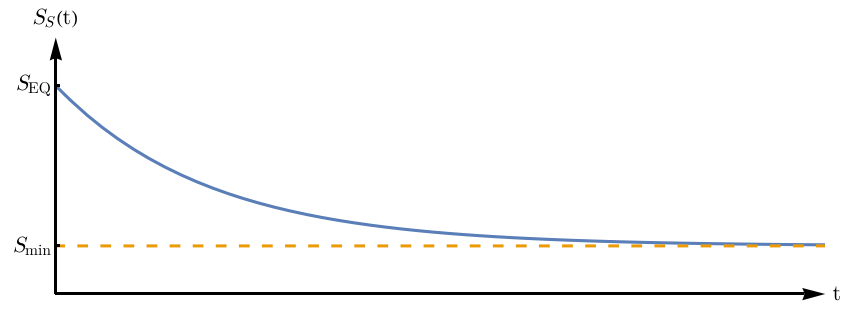
\includegraphics[width=12cm]{wykres3} 
\caption{Inducing lower entropy with heat flow.}
\label{Fig4} 
\end{figure}

This is of course consistent with the second law of thermodynamics as we're describing an open system.
It's easy to notice that the total entropy change is equal to $dS=dS_i \geq 0$ (for simplicity it was assumed that the heater and cooler don't act as producers of entropy).

\subsection{von Neumann entropy}

Although this work is meant to stay within the classical limit, it might be worth while to clear out the notion of entropy in quantum context.

The von Neumann entropy is defined as 

\begin{equation}
  S_{vN}= -\Tr(\hat{\rho} \log{\hat{\rho}}).
\end{equation}

For which the general form of the density matrix operator is

\begin{equation}
	\hat{\rho}=\sum_k p_k \ket{\psi_k}\bra{\psi_k} 
\end{equation}

in case of pure state $\ket{\psi}$ the density matrix is simply
\begin{equation}
  \hat{\rho} = \ket{\psi}\bra{\psi}
\end{equation}

and it is easy to verify that the entropy of a pure state is equal to zero. The entropy of mixed state is always greater than zero.
If the system is in a pure state, it will continue to be in a pure state as long as it stays isolated. For a mixed state, the degree of mixedness measured by the entropy will stay constant as long as it is isolated. This follows from the fact that the time evolution is unitary and the eigenvalues of the density operator therefore do not change with time.

An interesting question one might ask (and not really discussed in textbooks) is how the entropy changes after a measurement of a particle in many-body system which, initially, was in pure state.

Without loss of generalization let's consider an isolated system of two identical particles described solely by their momentum states.
In the scenario of two particles of identical momentum we can write the initial pure state as 
\begin{equation}
  \ket{2,0,0,...}
\end{equation}
which entropy is of course zero.  
In second quantization formalism the measurement of a particle is realized by the field operator $ \hat{\Psi}(x) =\sum_k \phi_k(x)\hat{a}_n$ which annihilates a single particle at position $x$.
Therefore after the measurement of particle at some position $x$, one particle is "virtually" removed from the system under consideration, but the system stays in pure state
\begin{equation}
  \hat{\Psi}(x)\ket{2,0,0,...}=\phi_1(x)\ket{1,0,0,...},
\end{equation}
which entropy is zero. It's important to notice though that our system lost a particle and therefore the systems before and after measurement are not equivalent! Of course, in reality the particle doesn't disappear. After determination of it's position by experiment ($\Delta x \to 0$), the uncertainty of it's momentum approaches infinity ($\Delta p \to \infty$), which means that we can reconstruct the state using a linear combination of states with \textit{any} value of momentum:

\begin{equation}
  c_1\ \ket{2,,0,...}+c_2\ \ket{1,1,0,...}+  c_3\ \ket{1,0,1,...}+...
\end{equation}
where the  squared modulus of the coefficients has to sum up to one ($ \sum_i \left| c_i \right|^2 = 1 $).

Now depending on the precision of the measurement we can recalculate entropy of course getting a value greater than zero. If we would perform the same analysis for a pure state of two particles in different states i.e. $ket{1,1,...}$ then we would obtain an increase of entropy even without accounting for the lost particle.
\todo{Correct also for correlated systems?}
This crude example gives a clear illustration of the fact that after \textbf{any} measurement the von Neumann entropy has to increase. However it's change is ultimately related to lost information about the system in the act of the measurement.

There's another interesting feature of quantum entropy, namely inequalities that it fullfills.
If we bipartite the system into subsystems $A$ and $B$ each containing it's own set of commuting observables, then in order to calculate the entropy $S_A$ of a subsystem $A$ we need to calculate the entropy with respect to density matrix traced over the other subsystem, namely
\begin{equation}
  \hat{\rho}^A = \Tr_B \hat{\rho} 
\end{equation}
then in general the following identities are satisfied

\begin{equation}
\begin{aligned}
	S(\rho) &\leq S_A + S_B	\\
	S(\rho) &\geq \left| S_A - S_B \right|
\end{aligned}
\end{equation}

The interpretation of the first inequality is that the full information about the states of the subsystems $A$ and $B$ will in general not be sufficient to give full information about the state of the total system $A+B$. Or in other words, when there are correlations between the two subsystems, these are not seen in the description of $A$ and $B$ separately. 

\section{Near-equilibrium thermodynamics}

\subsection{Concepts}
\subsection{Theory of fluctuations}
\subsection{Onsager relations}
%TODO Onsager START
[IN PROGRESS]
a term for entropy for open systems, an extension of Clausius entropy for isolated systems:

\begin{displaymath}
	dS=d_iS+d_eS
\end{displaymath}


Where \(d_iS\) is connected with entropy produced within the system and \(d_eS\) is the entropy transferred across the boundaries of the system.
The second law states that \(d_iS\geq 0\), so if a system is to stay in law entropy state it{'}s production must be compensated by an inflow of negative
entropy.

He then develops an explicit expression for entropy production, assuming that even outside equilibrium (but near) entropy depends only on the same
variables as at equilibrium ("local" equilibrium)

\begin{displaymath}
	P=\frac{d_iS}{dt}=\sum _{\rho } J_{\rho }X_{\rho }\geq 0
\end{displaymath}


where \(J_{\rho }\) are the rates of the various irreversible processes involved (chemical reactions, heat flow, diffusion$\ldots $) and \(X_{\rho
}\) are the corresponding, generalized forces (affinities, gradients of temperature, of chemical potentials$\ldots $). The flows are described using
different empirical laws (Fourier{'}s law, Fick{'}s law, etc.) 

\begin{displaymath}
	J_{\rho }=\sum _{\rho } L_{\rho \rho '}X_{\rho '}
\end{displaymath}

Onsager relations \(L_{\rho \rho '}=L_{\rho '\rho }\)
[IN PROGRESS END]
%TODO: Onsager END

\subsection{MinEP}

The most well known contribution of Ilya Prigogine to statistical physics, often called the Minimum Entropy Production (MinEP) principle, sprouts from the analysis of second order excess entropy around a steady state $ (\delta^2 S)_{ss} $. 

If we perturb the system around it's equilibrium state we obtain
\begin{equation}
  S=S_0 + \delta S + \frac{1}{2}\delta^2 S
\end{equation}

This quantity is than used as a Lyuponov function and has benefits over other (not necessarily all) Lyupanov functions one could define. 
Its macroscopic meaning is conserved independently of microscopic details of the system under consideration and is also independent of the nature of particular (possibly inhomogeneous) fluctuations.
It is important however, that this result holds only for steady states near-equilibrium. It is only near-equilibrium that the quantity $ (\delta^2 S)_{ss} $ generates probability of fluctuations, as Prigogine insisted in response to criticism \cite{Nicolis:1979cv}. 

The term "dissipative structures" was also coined by Prigogine.
In Prigogine's view the fluctuations are the trigger for the instabilities (or rather bifurcations in the equations of motion), which in turn give rise to spacetime structures, called poetically "dissipative structures". 
An often given example of instabilities leading to formation of structures are the Rayleigh-Bénard convection cells. In further part of this it will be demonstrated that this non-equilibrium system indeed lowers it's entropy.

\subsection{Green-Kubo relations}

\bibliographystyle{ieeetr}
\bibliography{Refs}


\end{document}